%% 
%% Copyright 2007, 2008, 2009 Elsevier Ltd
%% 
%% This file is part of the 'Elsarticle Bundle'.
%% ---------------------------------------------
%% 
%% It may be distributed under the conditions of the LaTeX Project Public
%% License, either version 1.2 of this license or (at your option) any
%% later version.  The latest version of this license is in
%%    http://www.latex-project.org/lppl.txt
%% and version 1.2 or later is part of all distributions of LaTeX
%% version 1999/12/01 or later.
%% 
%% The list of all files belonging to the 'Elsarticle Bundle' is
%% given in the file `manifest.txt'.
%% 
%% Template article for Elsevier's document class `elsarticle'
%% with harvard style bibliographic references
%% SP 2008/03/01

%\documentclass[preprint,12pt,authoryear]{elsarticle}  %default in the template
%\documentclass[preprint,10pt,authoryear]{elsarticle}

%% Use the option review to obtain double line spacing
%% \documentclass[authoryear,preprint,review,12pt]{elsarticle}

%% Use the options 1p,twocolumn; 3p; 3p,twocolumn; 5p; or 5p,twocolumn
%% for a journal layout:
%% \documentclass[final,1p,times,authoryear]{elsarticle}
%% \documentclass[final,1p,times,twocolumn,authoryear]{elsarticle}
 \documentclass[final,3p,times,authoryear]{elsarticle}
%% \documentclass[final,3p,times,twocolumn,authoryear]{elsarticle}
%% \documentclass[final,5p,times,authoryear]{elsarticle}
%% \documentclass[final,5p,times,twocolumn,authoryear]{elsarticle}

%% For including figures, graphicx.sty has been loaded in
%% elsarticle.cls. If you prefer to use the old commands
%% please give \usepackage{epsfig}

%% The amssymb package provides various useful mathematical symbols
\usepackage{amssymb}
%% The amsthm package provides extended theorem environments
\usepackage{amsthm}
\usepackage{amsmath}
\usepackage{color, colortbl}
\usepackage{amsmath}
\usepackage{siunitx}
%\usepackage{todonotes}
\usepackage{tabularx}
\usepackage[]{algorithm2e}
\usepackage{soul}
%\usepackage[colorinlistoftodos]{todonotes}

\usepackage{glossaries}

\usepackage{xargs}
\usepackage[pdftex,dvipsnames]{xcolor}
\usepackage[colorinlistoftodos,prependcaption,textsize=tiny]{todonotes}
\newcommandx{\unsure}[2][1=]{\todo[linecolor=red,backgroundcolor=red!25,bordercolor=red,#1]{#2}}
\newcommandx{\change}[2][1=]{\todo[linecolor=blue,backgroundcolor=blue!25,bordercolor=blue,#1]{#2}}
\newcommandx{\info}[2][1=]{\todo[linecolor=OliveGreen,backgroundcolor=OliveGreen!25,bordercolor=OliveGreen,#1]{#2}}
\newcommandx{\improvement}[2][1=]{\todo[linecolor=Plum,backgroundcolor=Plum!25,bordercolor=Plum,#1]{#2}}
\newcommandx{\thiswillnotshow}[2][1=]{\todo[disable,#1]{#2}}

\definecolor{light-gray}{gray}{0.9}

\usepackage{framed} % Framing content
\usepackage{multicol} % Multiple columns environment


\DeclareRobustCommand{\hlgreen}[1]{{\sethlcolor{green}\hl{#1}}}

\journal{TBD}
\makeglossaries


\begin{document}

%\runninghead{Nice et al.}

\title{Isolating the impacts of urban form and fabric from geography in assessing heat mitigation strategies }

\author[melb]{Kerry~A.~Nice\corref{cor1}}
\ead{kerry.nice@unimelb.edu.au}
\author[melb]{et al.}
%\author[melb]{Sachith Seneviratne}
%\author[melb]{Jasper S. Wijnands}
%\author[melb]{Jason Thompson}
%\author[melb,eng]{Mark Stevenson}
\cortext[cor1]{Principal corresponding author}
\address[melb]{Transport, Health, and Urban Design Hub, Faculty of Architecture, Building, and Planning, University of Melbourne, Australia.}
%\address[eng]{Melbourne School of Engineering; and Melbourne School of Population and Global Health, University of Melbourne, Australia.}







\begin{abstract}
\todo[inline]{TODO update}

Strategies for urban heat mitigation often make broad and non-specific recommendations (i.e. plant more trees) without accounting for local context. \todo{Negin Nazarian: suggest detailing what "local context" may refer to. 
for instance, regional geographic setting (lat/lon, distance from the coast, terrain) as well as background climate?
Nov 18, 2021 4:43 PM

Negin Nazarian: thinking about this again, the local context that I listed here is in fact not correct. Please see my lengthy note below. nonetheless, need to clarify} As a result, resources might be allocated to areas of lesser need over those where more urgent interventions are needed. Also, these interventions might return less than optimal results if local conditions are not considered. This project aims to assist with these interventions by providing a method to examine the urban heat profile of a city through an automated systematic approach. 

\todo[inline]{Negin Nazarian: May I suggest that we rephrase the emphasis of the paper? 
What I suggest is that we briefly note that canopy temperature and heat stress depend on 4 categories of parameters (taken from WMO work we are doing as well as Masson et al 2020): 1) built form, 2) natural and vegetated form (including soil, water, vegetation, and phenology of all), 3) urban "function" that covers human impacts, and 4) regional geographic settings.  Of these, (1) and (2) are often the focus of mitigation measures for urban heat. 
However, the interaction between these parameters, and their compounding effect on canopy T and HS, is non-linear. This complex interaction makes it hard to quantify the impact of mitigation measures in different cities with distinct urban form and functions and more importantly, distinguish this impact from regional geographical settings. 
To address this shortcoming, there is a need for a comprehensive set of sensitivity analyses that cover a combination of mitigation strategies with realistic built and natural forms existing in cities. So far, such sensitivity analyses are only done to a very limited extent  (focused on limited parameters or times of the day) motivating our current work to simulate XX many scenarios covering YY many parameters for moderate and extreme summer heat. This includes the most comprehensive  set of simulations that quantifies the sensitivity of canopy T and UTCI to a combination of design parameters. Using this method, the impact of mitigation strategies can be isolated from regional geographic settings (that has been impossible for instance with mesoscale simulations).
Nov 18, 2021 5:19 PM

Negin Nazarian: thinking about this again, the local context that I listed here is in fact not correct. Please see my lengthy note below. nonetheless, need to clarify
Nov 18, 2021 5:28 PM}


\end{abstract}

\begin{keyword}
micro-climate\sep 
urban morphology\sep
urban heat
\end{keyword}



\maketitle





\section{Introduction}
Heat in urban areas is the most dangerous natural hazard in Australia \citep{Coates2014}, with disproportionate risks falling on vulnerable populations such as elderly and the very young \citep{Nicholls2008}. Exposure to dangerous levels of heat stress is expected to increase by a factor of 5-10 by 2080 \citep{Coffel2018}, driven by more frequent, severe, and long-lasting heatwaves \citep{IPCC2013a}. The design of cities has exasperated these risks (through removing natural pervious land covers and increasing high-absorbent materials), resulting in increased heat stress for those who live in cities \citep{Coutts2012,Martilli2020}. The built environment design has altered urban energy balances in a number of ways \citep{Oke1982}. Anthropogenic heat wastes from buildings and transport and reduced shading through diminishing tree canopy cover result in larger amounts of net energy at street level. Meanwhile, the conversion of vegetated to impervious surfaces and reductions of available water in cities shift the urban energy balance away from latent heat (water evaporation) towards increased sensible heat (heat that can be felt) and heat storage in urban surfaces. 

In order to address the adverse effects of urban design on the thermal environments, mitigation strategies have deployed similar design strategies relying on modification of built form, fabric, and natural land covers in cities. Designing such mitigation strategies requires both an understanding of the processes driving excess heat (especially at a micro-climate level) and methods to identify areas of high risk in need of interventions. More importantly, being able to incorporate this knowledge into planning of future development means that new built areas can be designed as climate sensitive before the built form is locked in for decades to come. \todo{Negin Nazarian: suggest rewriting. Also, would be good to bring some examples (for instance systematic review of different mitigation strategies): 

https://iopscience.iop.org/article/10.1088/1748-9326/abdcf1/meta
Nov 18, 2021 5:41 PM}

Remote \todo{Negin Nazarian: hmmm this felt a bit out of the blue. my suggestion is to briefly note different metrics used for characterizing heat as well as heat mitigation impact. I'd start by canopy temperature, then note that spatial variability of it is low. Then note LST, but noting that it's not quite relevant, and lastly, detail MRT and UTCI which in many cases more important than temperature alone.
Nov 18, 2021 5:43 PM

Negin Nazarian: after noting this, you can create a hook between this paragraph and next, noting that canopy models are currently the best way to assess Ta and UTCI at the pedestrian/canopy level, while also providing an efficient way of obtaining spatial variabilities.
Nov 18, 2021 5:45 PM}
sensed land surface temperature (LST) has often been used to identify hotspots \citep{Aniello1995} or to evaluate cooling strategies \citep{Zhu2012a,Duncan2018,Manoli2019,Ossola2021}, however the validity of these results and the ability to link LST temperatures (measured at the top of the urban canopy) to thermal comfort at ground level can be limited and misleading  \citep{Coutts2016d}. As the shading provided by the urban canopy (both vegetation and urban structures) is a significant cooling mechanism \citep{Coutts2015,Lee2018,Krayenhoff2021}, these effects will not be captured in an above canopy assessment. However, obtaining under canopy observations of these heterogeneous environments is challenging, time consuming and limited in scale and resolution and to the observation time period \citep{Middel2019a}. In addition, the challenge of untangling the local weather conditions or topography from the influence of the urban form remains \citep{Potgieter2021}.

Modelling can be of use in assessing the thermal impacts of the ranges of urban arrangements and compositions. However, this also presents challenges. \todo{Negin Nazarian: since this is the method of this paper, I'd suggest phrasing this differently. perhaps focusing on the strengths and briefly noting challenges in the end?
Nov 18, 2021 5:50 PM} City-wide modelling at a micro-scale requires large investments in computation as well as the difficulty in obtaining high resolution data sources of urban form (land cover and building and vegetation heights and footprints) across cities and world-wide.

A number of efforts are under way to assemble these datasets. \todo{Negin Nazarian: which datasets?
Nov 18, 2021 5:51 PM} The World Urban Database and Access Portal Tools (WUDAPT) project \citep{Ching2018a} has been building an open data world-wide database of urban parameters necessary for climate modelling. Initial efforts have focused on building local climate zones (LCZ) \citep{Stewart2012b}, a standardised classification system to describe urban morphology typologies, providing local-scaled resolution coverage of wide areas of the world \citep{Demuzere2019}. While these initial efforts are not of sufficient resolution to support micro-scaled modelling, a pathway for higher resolution databases has been planned \citep{Ching2019}. \todo{Negin Nazarian: which does what? need to elaborate a bit more
Nov 18, 2021 5:52 PM} Other sources of urban information are becoming available, such as the commercial provider Geoscape \citep{Geoscape2020} which provides 2m resolution land cover coverage, as well as building and tree heights and footprints, of major Australian cities. However, currently there does not exist an open dataset with world-wide coverage at a scale sufficient for micro-scaled modelling.\todo{Negin Nazarian: suggest (a) creating a clear link to Masson et al 2020 (and the categorization made in the abstract), and (b) make the distinction in scales more clear (for instance, 2D vs 3D representation of cities, resolution, etc)}

Even with access to these data sources, performing human thermal comfort modelling of urban areas has many additional challenges. \todo{Negin Nazarian: This is why I think in the LST paragraph we should spell out different indictors of thermal environment vs thermal comfort} To capture all the influences of urban geometry and materials on human thermal comfort, especially the influences on mean radiant temperature \citep{Kantor2011} (a temperature that accounts for the thermal stresses on a person from both solar exposure and energy/heat radiating from nearby surfaces), modelling needs to be done at a micro-scale (that is, at a grid square or pixel resolution under 1km) \todo{Negin Nazarian: similarly, we certainly can benefit from detailing different scales in previous paragraphs.} and should account for the influence of vegetation and water features. While there are many urban models, there are few modelling options available at an appropriate scale and especially of models that account for all the elements of vegetation impacts and urban hydrology or that can explicitly calculate parameters needed to calculate human thermal comfort. Some of the available urban models include ENVI-met \citep{Bruse1999}, VTUF-3D \citep{Nice2018a}, SOLWEIG/UMEP \citep{Lindberg2018}, PALM \citep{Dominik2019}, canyon air temperature (CAT) \citep{Erell2006}, and OTC3D \citep{Nazarian2018}. 

For this study, VTUF-3D will be used. Previous efforts have utilised LCZs as the basis to provide the urban form input for climate modelling of specific areas \citep{stewart2014eval,Verdonck2018,Hammerberg2018,Masson2020,Emery2021}. However, this study will generate a full range of possible urban form combinations and then match the appropriate results back to each individual location as determined by its individual mix as determined by the high resolution Geoscape data across each city. \todo[inline]{Negin Nazarian: for both of these, need to articulate "why". Particularly the use of geoscape data vs LCZ, we should emphasize on the strength of this and more importantly, how you used such high-res dataset.
Nov 18, 2021 5:59 PM}

The aim of this study is therefore to devise a method to determine the influence of urban form on thermal comfort utilising a urban morphology data source and micro-climate modelling and apply it at a city-wide scale to allow identification of areas that could benefit from heat mitigation interventions as well as inform planning and development of new climate sensitive urban form. The first objective will be to model at a micro-scale the full range of representative combinations of urban form (mixes of land cover and urban and vegetative structure). The second objective will be to use these results to determine the importance and relative influence of each feature type on thermal performance. The final objective will be to build the results back up to a city-wide assessment of thermal comfort due to urban form.\todo[inline]{Negin Nazarian: after deciding on the objectives noted in the abstract, suggest modifying this as well.
Nov 18, 2021 6:01 PM}






\section{Methods}\label{sec:methods}
\todo[inline]{Negin Nazarian: perhaps we can add a workflow? I dont know if it's common in Nature publications though...}


\subsection{Scenario generation}\label{sec:methodsgen}
Geoscape \citep{Geoscape2020}, data from Public Sector Mapping Agency (PSMA) Australia, provides 2 meter resolution land cover (road, building, grass, bare earth, etc) as well as building and tree footprints and heights. Representative ranges of surface covers and tree and building heights and footprints were calculated for Melbourne. \todo{Negin Nazarian: This puzzled me a bit. You mention that you used Geoscape to inform the modeling, but most parameters are varied between 0-100\%. So how did the "representative ranges" come into play?} From these, 9814 model domains were created with all iterations (by 5\% increments) of fractions of trees, grass, buildings and streets, as well as heights of buildings (from 0 to 49 meters) and vegetation (from 0 to 20 meters in 0.5m increments) (Figure \ref{fig:scenarios}). These domains were created of 100$\times$100m with 5m resolution grids. Additionally, surface fractions and average building and vegetation heights were calculated for 100$\times$100m locations across Melbourne, Sydney, Adelaide, Brisbane, and Perth. \todo[inline]{Negin Nazarian: need to explain better. can't quite get how 10,000 cases are generated!}


\begin{figure*}
\centering
\includegraphics[page=15,trim={70 380 60 390},clip,scale=0.65]{Figures/Figures6.pdf}
\caption{\bf Creation of VTUF-3D scenarios for 9814 variations of parameters across representative ranges in Melbourne.}
 \label{fig:scenarios}
\end{figure*} 




\subsection{VTUF-3D}\label{sec:methodsvtuf}
VTUF-3D \citep{Nice2018a} was used as the micro-climate modelling tool for this study. VTUF-3D is a urban micro-climate surface energy balance model that incorporates vegetation physiological processes and shading effects. The model provides output of a canyon averaged air temperature ($T_{can}$) as well as values for each surface of surface temperature ($T_{surf}$), mean radiant temperature ($T_{mrt}$), and the universal thermal climate index ($UTCI$) (Figure \ref{fig:vtufresults}). All the scenarios were run with a 5m resolution and were forced by the observations of Preston in Melbourne from \cite{Coutts2007} over the days February 9-13, 2004. Additional scenario runs were performed for February 13-16, 2004 using the same forcing data source. As temperatures reached 36\SI{}{\degreeCelsius} on February 14th, these will provide extreme heat days.\todo[inline]{Negin Nazarian: please add some notes re validation of VTUF3d
Nov 18, 2021 6:07 PM}

\begin{figure*}
\centering
\includegraphics[page=2,trim={75 240 60 240},clip,scale=0.35]{Figures/PresentationImages.pdf}
\caption{\bf Example VTUF-3D results of UTCI at ground surface levels for a Melbourne scenario.}
 \label{fig:vtufresults}
\end{figure*} 

\todo[inline]{TODO, will the extreme days be necessary? Lots of those runs failed so the data is much patchier than the more average days.  Negin Nazarian: oh interesting. curious to know why they failed? I find it really interesting to have the hot days, since most mitigation scenarios are proposed with extreme weather in mind.}

An analysis time was used of 4 pm of February 12, 2004 for many parts of the analysis. The current forcing conditions at that point were downward shortwave (\gls{kdown}) of 501.7$Wm^{-2}$, downward longwave (\gls{ldown}) of 365.1$Wm^{-2}$, air temperature of 25.9\SI{}{\degreeCelsius}, vapour pressure of 1.16 $mb$, wind at 173$^{\circ}$ of 5.4 $ms^{-1}$ and air pressure of 995.5$mb$. Energy balance parameters for net radiation (\gls{qstar}), sensible fluxes (\gls{qh}), ground flux (\gls{qg}), and latent heat (\gls{qe}) were also extracted, as well as shortwave and longwave up (\gls{kup} and \gls{lup}) (all in $Wm^{-2}$) and canyon wind speed ($U_{road}$) (in $ms^{-1}$).\todo[inline]{Negin Nazarian: can we put this in a table?}

\todo[inline]{TODO, do I need more detail about the rest of the days/times? Some graphs of the conditions?  Negin Nazarian: I believe so. overall, you need some description of why this is selected (representing average warm day), how many days the simulations are ran and why this is appropriate, and when the result are focused on}



\subsection{Parameter analysis}\label{sec:methodsparam}\todo[inline]{Negin Nazarian: perhaps sensitivity analyses? overall, need a bit of intro in the beginning of some sections (what you wish to achieve and why)}
% analysis
% ProcessMCZResults.java
% -  temperature distributions at 0m created for each completed run
%  All surfaces at 0m for each timestep, temperatures and counts of for Tsfc, Tmrt, and UTCI.
%  Ta is single value (canyon averaged) for each domain
% - All runs are combined into single data file for each timestep
%     contains temperatures and energy fluxes


Results  at ground level (all in $^{\circ}$C) from the 9814 completed model runs were extracted and a domain mean value calculated for each hourly timestep for \gls{tsfc}, \gls{tmrt}, and \gls{utci}. \todo{Negin Nazarian: don't you also show spatial distribution of UTCI later?
Nov 18, 2021 6:10 PM

Negin Nazarian: I suggest rewording and noting spatial and temporal distribution of X,Y, Z is captured at ground level, while canopy temperature assumes well mixed air in the canopy and therefore only temporal evolutions are outputted
Nov 18, 2021 6:11 PM} VTUF-3D generates a single canyon averaged air temperature (\gls{tcan}). Additionally, domain averaged energy flux values were extracted, including latent fluxes (\gls{qe}), sensible fluxes (\gls{qh}), net radiation (\gls{qstar}), ground fluxes (\gls{qg}), shortwave up (\gls{kup}), shortwave down (\gls{kdown}), longwave up (\gls{lup}), and longwave down (\gls{ldown}). Hourly results were combined and indexed by their unique parameter ranges.\todo{Negin Nazarian: not clear?}

\todo[inline]{Double check whether it was 9814 scenarios and change throughout.}

\subsection{Feature importance}\label{sec:methodsfeat}
%
% Feature importance
% /media/kerryn/87d9469d-56aa-4a1f-a62d-5f03d7599bbf/Data/VTUF-3D/Output/FeatureImportance/rf_all_runszslice.py
% also rf_all_runszslicemcz4.py (for heatwave)
% plotted with plot_daily_feature_imp.R, now plot_daily_feature_imp2.R (for just one day)
% feature_imporantance from RandomForestClassifier was used from scikit-learn \citep{scikit-learn}
% determine feature importance for paramaters of percentages of grass, trees, buildings, and roads, as well as average vegetation and building heights for Tair, Tsfc, Tmrt, and UTCI.

A feature importance analysis was performed using the Random Forest Classifier from  scikit-learn \citep{scikit-learn}. Ranks of feature importance were determined for each temperature type (\gls{tcan}, \gls{tsfc}, \gls{tmrt}, and \gls{utci}) for the four surface fraction parameters (grass, trees, buildings, and roads) as well as average vegetation and building heights at each hour during the simulations.\todo[inline]{Negin Nazarian: as noted before, a bit of explanation why this is needed and what it means?}


\subsection{Temperature trends due to surface fractions and average heights}\label{sec:methodstempvspercent}

% cd /home/kerryn/git/2020-07-Frontiers-UrbClimInformatics/Analysis/Figures
% box_montage_reverse_zslice.sh
% plot_box_unclustered_tempRangeszSlice.py -> plot_box_reverse_6zSlice.py
% for heatwave:
%  box_montage_reverse_mcz4.sh
%      plot_box_unclustered_tempRangesMCZ4.py -> plot_box_reverse_6MCZ4.py
% matplotlib used to plot hourly results for all scenarios for 4 temperature types
%  box plots made of temperatures vs percentages (by 10 %) of surfaces (tree, grass, building, road) and ave heights (by 0.4m) of vegetation and buildings
%  background colors of each plot were tinted by levels of feature importance.
     % then r2_boxplots.py
     % R2 calculated for each parameter over dinual cycle and plotted against the other parameters
     % Nope, didn't use R2. This is the replacement:
% plot_box_reverse_zslice_per_10percent.py (called from 'bash ten_percent_fraction_plots.sh')
%     heatwave plot_box_reverse_zslice_per_10percentMCZ4.py (called from 'bash ten_percent_fraction_plotsMCZ4.sh')
% plot_box_10percent_r2_replacement.py (to generate the data file)
% plot_10percent_increases_cycle.R
% switch to absolute values instead of increases
% plot_box_absolute_10percent_r2_replacement.py
% plot_10percent_absolute_cycle.R
%
%  plot box per 10 % used pandas describe and groupby to find the mean temperature increases per 10 % fraction increases or 0.8m height increases.
%    These were plotted at a few specific times comparing temperature increases vs surface fractions.
%  To replace R2, a full day's data was split into panels for each surface type and the differences plotted individually for each 10 % increment.

To determine the trends of the four temperature types (\gls{tcan}, \gls{tsfc}, \gls{tmrt}, and \gls{utci}), Matplotlib \citep{Hunter2007} was used to generate box plots of modelled temperature results vs surface types (tree, grass, building, road) grouped by 10\% ranges as well as average building and vegetation heights (in 0.8m ranges). The backgrounds of each plot were tinted in green according to the parameter's calculated level of feature importance (a range of 0-1).

%To explore the trends associated with each surface fraction type over a diurnal cycle, the $R^{2}$ of modelled temperature vs. surface fraction percentage or average building or vegetation heights was calculated for each hour for each of the six parameters and four temperature types and plotted as a line graph. 

In addition, mean temperatures were calculated for each temperature type and fraction percentages and heights using pandas \citep{reback2020pandas} describe method and groupby of 10\% increments of surface fractions or 0.8 meter average heights. Then temperature differences between increasing fractions and heights were calculated and plotted across the entire diurnal cycle of 12 Feburary 2004.



\subsection{Distributions of temperatures across a diurnal cycle}\label{sec:methodsdist}
%
% ridge plots, ggridge_plots.R
%   sample scenarios were selected (that represented some of the most common urban arrangments)
%   hourly distributions on Feb 12 of Tsfc, Tmrt, and UTCI (Ta is only canyon averages) using R ggplot ggridges
% 

A number of scenarios were selected that represented frequent (and the range of) urban morphologies found in Melbourne and hourly distributions over a diurnal cycle (of February 12th) using ggridges \citep{ggridges}. Temperatures plotted were \gls{tsfc}, \gls{tmrt}, and \gls{utci}. \gls{tcan} is a single canyon average so does not have a distribution.


\subsection{City scale heat maps from micro-climate modelled results}\label{sec:methodsheatmaps}
% city heat maps
%  the vtuf scenarios used forcing (and range of urban morphologies) from Melbourne (Preston) Coutts 2007
%  completed model results were matched back to locations across Melbourne by matching the modelled parameters 
%   of surface fractions and heights to the actual parameters of those locations.
%  resulting heat maps of Ta, Tsfc, Tmrt, and UTCI were visualised in QGIS.
%  Tsfc results were compared to CSIRO LST maps generated by \citep{Devereux2017} and visialised in QGIS.
%  In addition, model results were matched to locations in Sydney, Perth, Brisbane, and Adelaide to generate heatmaps
%  Correlations between differences and surface fractions 
%  /home/kerryn/git/2020-07-Frontiers-UrbClimInformatics/Analysis/Figures/GISMap
%  correlations.R

City-wide heat maps of \gls{tcan}, \gls{tsfc}, \gls{tmrt}, and \gls{utci} were generated from the 9814 modelled scenario results. Each model run was forced by the observations of Preston in Melbourne from \cite{Coutts2007} over the days February 9-14, 2004. The actual urban morphology parameters calculated from the Geoscape data were matched to the modelled scenario with the closest matching parameters of surface fractions and average heights for each 100$\times$100m location in Melbourne and visualized using the sf package \citep{Pebesma2018} in R. Locations with greater than 10\% surface fraction of water were removed from the results as VTUF-3D does not currently model water bodies. These resulting heatmaps show a city-wide assessment of thermal performance due to urban form but is independent of local weather conditions (i.e. ocean breezes vs. calm inland conditions) and topography (differing elevations across the cities). 

In addition, the same modelled results were matched to locations across Sydney, Perth, Brisbane, and Adelaide to generate city-wide urban form heatmaps for each of these cities.  \gls{tsfc} heatmap results were compared to the land surface temperature (LST) maps of Melbourne, Sydney, and Perth from Landsat 8. All Landsat 8 imagery corresponds to 10am local time. Imagery was selected of cloudless conditions for each city that most closely matched forcing conditions. Melbourne images were from December 11, 2018  (air temperatures minimum and maximums of 22 and 26\SI{}{\degreeCelsius}) and December 27, 2018  (air temperatures minimum and maximums of 15 and 39\SI{}{\degreeCelsius}). Sydney images were from March 11, 2019  (air temperatures minimum and maximums of 22 and 26\SI{}{\degreeCelsius}) and 19 January 2018  (air temperatures minimum and maximums of 18 and 31\SI{}{\degreeCelsius}). Perth images were from March 29, 2019  (air temperatures minimum and maximums of 13 and 27\SI{}{\degreeCelsius}) and 25 February 2019  (air temperatures minimum and maximums of 19 and 37\SI{}{\degreeCelsius}). LST results were visualised in QGIS \citep{QGIS2009}.


\section{Results}\label{sec:results}

\subsection{Temperature trends across fractions and feature importance}\label{sec:resulttrends}

%The range of ground level mean results from 9814 scenarios for four temperature types (\gls{tcan}, \gls{tsfc}, \gls{tmrt}, and \gls{utci}) at varying surface fractions of grass, trees, buildings, and roads and average heights of vegetation and buildings are presented in Figures \ref{fig:box0}, \ref{fig:box5}, \ref{fig:box14} on February 12, 2004 at 12am, 5am, and 2pm respectively.














The range of average results from 9814 scenarios for two temperature types (\gls{tcan} and \gls{utci}) at varying surface fractions of grass, trees, buildings, and roads and average heights of vegetation and buildings are presented in Figures \ref{fig:box5a}, \ref{fig:box14a} on February 12, 2004 at 5am and 2pm respectively. Note, there are a small number of scenarios with very high fractions of a surface type (80-100\%) compared to those with very small fractions, as a scenario with, as an example, 90\% grass means there are only a small number of combinations to use the remaining 10\% fractions. Although, for each of these surface fraction combinations, there are a range of scenarios with varying vegetation and building heights.


% used 
%  % cd /home/kerryn/git/2020-07-Frontiers-UrbClimInformatics/Analysis/Figures
% plot_box_unclustered_tempRangeszSlice_final.py -> plot_box_reverse_6zSlice_final.py
\begin{figure*}
\centering
\includegraphics[page=1,trim={62 305 62 305},clip,scale=1.0]{Figures/Figures6.pdf}
\caption{\bf Surface fractions percentages (trees, grass, buildings, and streets) and average heights (vegetation and building) vs. \gls{tcan} (top) and \gls{utci} (bottom) for February 12, 2004, 5am (left) and 2pm (right). Feature importance for each temperature type is indicated by the green background tinting.}
 \label{fig:box5a} \label{fig:box14a}
\end{figure*} 



\todo[inline]{Some of below should change, now that I've taken out 12am and just have 5am and 2pm. Also, only using TCAN and UTCI now, remove TSFC and TMRT.}


During the nighttime (12am and 5am), there is a narrow range of \gls{tcan}, from approximately 15.3-16.3$^{\circ}$C. Increasing fractions of trees have very little effect at 12am and slight reductions of approximately 0.1$^{\circ}$C when increasing trees from 0 to 100\%. Increasing vegetation height has an almost identical impact at nighttime. Increasing grass fractions has a slight warming impact of about 0.3$^{\circ}$C. Increasing building heights has an almost identical effect. Increasing building and street fractions has a mostly neural effect but at dawn (5am), the increasing street fractions start to have a very slight warming impact (0.3$^{\circ}$C). 

At nighttime, trends of \gls{utci}, which include the influences of \gls{tsfc} and \gls{tmrt}, show decreases of approximately 2.5$^{\circ}$C as fractions of trees and buildings and vegetation heights increase. \gls{utci} increases are seen of approximately 3.0$^{\circ}$C as grass fractions and building heights increase and 1.5$^{\circ}$C as street fractions increase.

At 2pm, at the warmest time of the day, increasing tree and building fractions and increasing vegetation height continue to provide some \gls{tcan} temperature reductions of 1-2$^{\circ}$C. Grass fractions and building heights increases show an initial reduction towards the middle fraction ranges then an increase at the higher ranges, with a reduction in the middle ranges of approximately 1$^{\circ}$C. Increases in street fractions however show a rapid increase in \gls{tcan} temperatures of approximately 3$^{\circ}$C as street fractions approach 80\% and another 3$^{\circ}$C at 90\%.

At 2pm, trends of \gls{utci} amplify the trends seen with \gls{tcan}. Increases in street fractions show increases of approximately 6$^{\circ}$C as street fractions approach 80\% and another 6$^{\circ}$C at 90\%. Increasing grass and building heights shows increases of 5$^{\circ}$C as fractions increase. Increasing tree and building fractions and tree heights show reductions in temperatures of approximately 5$^{\circ}$C.




In Figure \ref{fig:tcanday}, \gls{tcan} temperatures are shown for ranges of fractions and heights across the diurnal cycle of 14 February 2004. In these, small differences (1$^{\circ}$C) are seen at night-time, with larger ranges seen with street fractions and to a lesser degree with building fractions and building heights. After dawn, the differences begin to increase and reaching a peak at mid-day with maximum differences of approximately 5$^{\circ}$C with grass, tree, building fractions and building and vegetation heights. Differences at mid-day reach maximum divergences of 10 and 15$^{\circ}$C as street surface fractions reach 80 and 90\% respectively.

% run with plot_10percent_absolute_cycle_final.R
\begin{figure*}
\centering
\includegraphics[page=2,trim={90 238 90 238},clip,scale=0.95]{Figures/Figures6.pdf}
\caption{\bf Mean \gls{tcan} outcomes clustered by 10\% surface fraction ranges of a) grass, b) streets, c) trees, and d) buildings and e) average vegetation and f) average building heights clustered by 0.8m increases over a diurnal cycle of February 12, 2004.  }
 \label{fig:tcanday}
\end{figure*}


For \gls{utci} (Figure \ref{fig:utciday}) which include the influence of \gls{tsfc} and \gls{tmrt}, the night-time ranges show wider differences, with all fractions and heights showing a difference of 2-3$^{\circ}$C between the lowest and highest amounts of fractions and heights. These difference remain roughly similar through dawn and until about 8am. Street fractions are the exception and show even wider divergences (5$^{\circ}$C and more) starting at 6am. After 6am, differences widen to 5$^{\circ}$C for building fractions and building heights and 10$^{\circ}$C for tree and grass fractions and vegetation heights. Meanwhile, differences for street fractions grow to nearly 15$^{\circ}$C for 80\% and over 20$^{\circ}$C for 90\%.

\todo[inline]{TODO, this all seems a bit dense. Would a table help?}







% run with plot_10percent_absolute_cycle_final.R
\begin{figure*}
\centering
\includegraphics[page=3,trim={90 238 90 238},clip,scale=0.95]{Figures/Figures6.pdf}
\caption{\bf Mean \gls{utci} outcomes clustered by 10\% surface fraction ranges of a) grass, b) streets, c) trees, and d) buildings and e) average vegetation and f) average building heights clustered by 0.8m increases over a diurnal cycle of February 12, 2004. }
 \label{fig:utciday}
\end{figure*}


Analysis of feature importance shows that building fractions and building heights are most significant for \gls{tcan} (Figure \ref{fig:featimpttcan}a) at night while building fractions and building heights are slightly more important than grass and streets and trees and vegetation heights are of the lowest importance for \gls{utci} (Figure  \ref{fig:featimptutci}b). During the daytime, street fractions are of the highest importance for both \gls{tcan} and \gls{utci}.


\begin{figure*}
\centering
{\tiny a)}\includegraphics[page=16,trim={55 275 50 295},clip,scale=0.45]{Figures/Figures6.pdf}
{\tiny b)}\includegraphics[page=17,trim={55 275 50 295},clip,scale=0.45]{Figures/Figures6.pdf}\\
\caption{\bf Feature importance in a) \gls{tcan} and b) \gls{utci} for the four surface fractions of streets, buildings, trees, and grass and average heights of vegetation and buildings across February 12, 2004.}
\label{fig:featimpttcan}
\label{fig:featimptutci}
\end{figure*}




\subsection{Distributions of temperatures across a diurnal cycle}\label{sec:resultsdist}


Figure \ref{fig:dist1}  show the \gls{utci} distributions for a number of selected scenarios across the 24 hours of February 12, 2004. The preceding results (Section \ref{sec:resulttrends}) is based on mean values, averaged across the ground level results across each domain. However, different mixes of surface fractions and average heights result in widely varying distributions of temperatures (all in $^{\circ}$C). 


Panel A presents a scenario with very low fractions of roads and buildings and as a result show \gls{tsfc} temperatures mostly clustered in the lower ranges across day and night and very few locations that exceed the mid 20s during the day. Panel B shows a scenario with a moderate amount of streets and buildings (20\% and 30\%), but the height of the buildings and the vegetation cover yields similar results to Panel A. Panel D shows a strong shift towards predominately hotter \gls{utci} temperatures (30$^{\circ}$C) across the entire domain during the daytime (also reflected in the median), while Panel C shows a similar distribution but the median is much lower (in the lower 20s$^{\circ}$C).
\todo[inline]{say a bit more about the distributions and the different fractions.}

%Figures \ref{fig:dist1}, \ref{fig:dist3}, and \ref{fig:dist5} present scenarios As the fractions of road and buildings increase, especially in Figure \ref{fig:dist4}, where road and building fractions are 30 and 40\% respectively, the distributions shift strongly during the day away from locations with surface temperatures in the mid 20s to many more locations with surface temperatures in the 40s and even 50s and above.

%\todo[inline]{Change the above discussion since order of the panels in the figure has changed. And a red line for median has been added, so the medians in c and d are quite different even though the distributions look kind of similar. }
 
 
\begin{figure*}
\centering
\fbox{
a)\includegraphics[page=4,trim={60 225 40 251},clip,scale=0.47]{Figures/Figures6.pdf}
}
\fbox{
b)\includegraphics[page=6,trim={150 225 40 251},clip,scale=0.47]{Figures/Figures6.pdf}
}
\\
\fbox{
c)\includegraphics[page=9,trim={60 225 40 251},clip,scale=0.47]{Figures/Figures6.pdf}
}
\fbox{
d)\includegraphics[page=10,trim={150 225 40 251},clip,scale=0.47]{Figures/Figures6.pdf}
}
\caption{\bf Distribution of \gls{utci} across February 12, 2004 for scenarios a) 50\% grass, 49.99\% trees, 0.01\% road, 0\% building, average vegetation height of 4m, and average building height of 0m, b) 29\% grass, 69\% trees, 1\% road, 1\% building, average vegetation height of 0.5m, and average building height of 5m, c) 40\% grass, 10\% trees, 20\% road, 30\% building, average vegetation height of 2m, and average building height of 14m, and d) 19\% grass, 20\% trees, 21\% road, 40\% building, average vegetation height of 1m, and average building height of 9m. Red line indicates hourly median temperature. Insert shows percent fractions of surface types.}
 \label{fig:dist1}
\end{figure*}





\section{Discussion}\label{sec:discussion}








\subsection{City scale heat maps from micro-climate modelled results}\label{sec:resultsheatmaps}



\todo[inline]{TODO, double check that is 4pm not 2pm}

Figure \ref{fig:TaMelb} shows city-wide heat maps of \gls{tcan} and \gls{utci} in Melbourne at 2pm on February 12, 2004 constructed by matching the closest matching parameters for each locations from the 9814 modelled scenario results. A narrow range of air temperatures are seen across most of the city, closely aligned to the modelling forcing temperature of 25.9\SI{}{\degreeCelsius}. Higher temperatures can be seen in areas corresponding to higher fractions of roads and to a lesser degree of buildings. No particular reductions of air temperatures are seen in areas corresponding to higher levels of trees or grass surface fractions. Fractional breakdowns of surfaces types across Melbourne are shown in Figure \ref{fig:melfracs}. 

\begin{figure*}
\centering
a)\includegraphics[page=18,trim={63 421.25 370 215},clip,scale=1.3]{Figures/Figures6.pdf}
b)\includegraphics[page=18,trim={234 220 195 420},clip,scale=1.3]{Figures/Figures6.pdf}
\caption{\bf a) \gls{tcan} and b) \gls{utci} heatmaps on February 12, 2004 at 2pm generated by matching the closest matching parameters of surface fractions and average heights for each 100$\times$100m location in Melbourne from 9814 modelled scenario results (in \SI{}{\degreeCelsius}). }
 \label{fig:TaMelb}  \label{fig:utciMelb}
\end{figure*}

\begin{figure*}
\centering
\includegraphics[page=19,trim={55 215 200 215},clip,scale=1.0]{Figures/Figures6.pdf}
\caption{\bf Surface fractions of a) grass, b) trees, c) buildings, and d) streets across Melbourne. TODO:Are these needed for the discussion or are they supplementary?}
 \label{fig:melfracs}
\end{figure*}


Wider ranges of surface temperatures are seen across Melbourne. Some slight reductions of surface temperatures (below the forcing air temperature) are seen in areas that correspond to higher fractions of grass and of trees. However, strong increases in surface temperatures in areas with higher fractions of street surfaces, even starting at lower street fraction levels of 30\% and above.  In addition, very strong increases in surface temperatures can be seen in areas with very high street surface fractions, for example Melbourne Airport in the north west, the central business district (CBD) in the city centre, and Moorabbin Airport in the city south east.

Figure \ref{fig:Melb_TSFC12_85} presents a comparison of modelled \gls{tsfc} to Landsat 8 LST data. Panel a for the figure shows Landsat 8 imagery captured on cloudless days that mostly closely correspond to the modelled conditions, 10am December 11, 2018 when local conditions of air temperature on this day were minimum and maximum of 22 and 26\SI{}{\degreeCelsius}. Panel b for shows \gls{tsfc} created from modelled results at 10am on February 12, 2004 and February 14, 2004. 

In comparing the constructed \gls{tsfc} heat maps with the LST imagery, some observations can be made. However note, the two datasets measure different things and might not be entirely comparable. LST observations are captured by satellite and correspond to temperatures at the top of the urban canopy (i.e. the tops of trees and buildings) while the modelled \gls{tsfc} corresponds to ground surface temperatures and will generally be cooler as they include areas that are shaded by tree canopies and buildings. In addition, LST observations are influenced by additional factors than just the urban form including topography and localised weather conditions. In Figure \ref{fig:Melb_TSFC12_85}a, the cooler locations in the LST observations mostly include locations immediately off the coast and in the eastern fringes of Melbourne, the Dandenong Ranges which range from 500m to over 1000m in elevation, while the majority of central and inner Melbourne is under 100m in elevation. The main differences between the LST observations and the modelled results are strongly related to the surface fraction types, which a strong correlation between the differences and building and street fractions and a strong negative correlation with grass surface fractions. 

\begin{figure*}
\centering
a)\includegraphics[page=13,trim={75 225 195 245},clip,scale=0.54]{Figures/Figures6.pdf}
b)\includegraphics[page=11,trim={63 230 220 250},clip,scale=0.56]{Figures/Figures6.pdf}
\caption{\bf a) Landsat 8 land surface temperature (\SI{}{\degreeCelsius}) captured 10am December 11, 2018. Local conditions of air temperature on this day were minimum and maximum of 22 and 26\SI{}{\degreeCelsius}. b) Modelled \gls{tsfc} (\SI{}{\degreeCelsius}) on February 12, 2004 at 10am generated by matching the closest matching parameters of surface fractions and average heights for each 100$\times$100m location in Melbourne from 9814 modelled scenario results.}
 \label{fig:Melb_TSFC12_85}
\end{figure*}


Using the 9814 modelled scenario results, heat maps of \gls{tcan} and \gls{utci} (Figure \ref{fig:TaSyd}) were created for Sydney for February 12, 2004 at 2pm by matching the closest matching parameters, as calculated from Figure \ref{fig:sydfracs}, for each location. In Figure \ref{fig:Sydney-Landsat-LST-11-03-2019}, panel a shows cloudless Landsat 8 observations from 10am March 11, 2019 (local conditions of air temperature on this day were minimum and maximum of 22 and 26\SI{}{\degreeCelsius}) while panel b shows \gls{tsfc} heatmaps created from modelled results at 10am on February 12, 2004. 

The results are similar to those from Melbourne. Ranges of \gls{tcan} are generally very narrow with small localised hot spots. The LST observations reflect a different topography than Melbourne with a larger influence of coastal features and a smaller range of elevations. Much of the central city is under 100m and only approaching 200m in the north east areas. The areas with higher ranges of LST are concentrated in the agricultural western regions of the city (with very high percentages of grass/low vegetation land cover fractions). Similar to Melbourne, correlations between differences between LST and \gls{tsfc} are strongly negatively correlated with grass fractions but somewhat less correlated with building and street fractions.

%Using the 9814 modelled scenario results, heat maps of \gls{tcan} and \gls{tsfc} (Figure \ref{fig:TaPerth}) were created for Sydney for February 12, 2004 at 2pm by matching the closest matching parameters, as calculated from Figure \ref{fig:perthfracs}, for each location. In Figures \ref{fig:Perth_TSFC12_85} and \ref{fig:Perth_TSFC14_85}, cloudless Landsat 8 observations from 10am March 29, 2019 (local conditions of air temperature on this day were minimum and maximum of 13 and 27\SI{}{\degreeCelsius}) and 10am February 25, 2019 (local conditions of air temperature on this day were minimum and maximum of 19 and 37\SI{}{\degreeCelsius}) are presented and compared to \gls{tsfc} heatmaps created from modelled results at 10am on February 12, 2004 and February 14, 2004. 


%Ranges of \gls{tcan} are generally narrow with small localised hot spots (including the Perth Airport in the center east of the city). The topography of Perth is much less varied than Melbourne and Sydney, with the majority of the city under 50m in elevation and only rising above 100m in the eastern fringes. Much of the city is influences by coastal features. Much of the city is low density residential only becoming mixed with low vegetation/grassland reserves in the southern sections of the city. Similar to Melbourne, correlations between differences between LST and \gls{tsfc} are strongly negatively correlated with grass fractions and strongly correlated with building and street fractions.

\begin{figure*}
\centering
a)\includegraphics[page=2,trim={63 421.25 370 215},clip,scale=1.3]{Figures/Figures7.pdf}
b)\includegraphics[page=2,trim={234 220 195 420},clip,scale=1.3]{Figures/Figures7.pdf}
\caption{\bf a) \gls{tcan} and b) \gls{utci} heatmaps on February 12, 2004 at 2pm generated by matching the closest matching parameters of surface fractions and average heights for each 100$\times$100m location in Sydney from 9814 modelled scenario results (in \SI{}{\degreeCelsius}).  }
 \label{fig:TaSyd} \label{fig:utciSyd}
\end{figure*}


\begin{figure*}
\centering
\includegraphics[page=1,trim={55 215 200 215},clip,scale=1.0]{Figures/Figures7.pdf}
\caption{\bf Surface fractions of a) grass, b) trees, c) buildings, and d) streets across Sydney. TODO:Are these needed for the discussion or are they supplementary?}
 \label{fig:sydfracs}
\end{figure*}

%16 Sydney-Landsat-LST-11-03-2019  %//  11/03/2019	22	26
\begin{figure*} 
\centering
a)\includegraphics[page=14,trim={65 245 245 240},clip,scale=0.53]{Figures/Figures6.pdf}
b)\includegraphics[page=12,trim={60 220 210 225},clip,scale=0.48]{Figures/Figures6.pdf}
\caption{\bf a) Landsat 8 land surface temperature (\SI{}{\degreeCelsius}) captured 10am March 11, 2019. Local conditions of air temperature on this day were minimum and maximum of 22 and 26\SI{}{\degreeCelsius}. b) Modelled \gls{tsfc} (\SI{}{\degreeCelsius}) on February 12, 2004 at 10am generated by matching the closest matching parameters of surface fractions and average heights for each 100$\times$100m location in Sydney from 9814 modelled scenario results.}
 \label{fig:Sydney-Landsat-LST-11-03-2019}
 \label{fig:Sydney_TSFC12_85}
\end{figure*}

Through systematic micro-climate modelling of the full range of surface fractions and average heights across Melbourne, the importance and relative influence of each feature type on the temperature types of \gls{tcan}, \gls{tmrt}, \gls{tsfc}, and \gls{utci} was examined. For \gls{tcan}, at night time, there was a narrow range of temperatures, of approximately 1.0\SI{}{\degreeCelsius}. Increasing fractions of trees had a limited impact at midnight and contributed to a very slight reduction (0.1\SI{}{\degreeCelsius}) at dawn. Increasing grass and building heights had a small warming impact (0.3\SI{}{\degreeCelsius}). Increasing street fractions contributed to a warming effect (0.3\SI{}{\degreeCelsius}) at dawn. Building fractions and building heights were found to be the most significant features at night time.

During the daytime, the most important feature was the fraction of streets. Street fractions of 80 and 90\% can drive \gls{tcan} increases of up to 10 and 15\SI{}{\degreeCelsius} while reductions are seen of about 5\SI{}{\degreeCelsius} when increasing grass and tree fractions from 0 to 100\%. These results help futher describe findings of \cite{Emery2021} in their observations of the influence of different LCZ classes on air temperature. They found that the LCZ classes with the warmest temperatures were those dominated by artificial, mineral, and impervious surfaces, as well as LCZ classes with vegetation were the coolest. However, they were not able to characterise the expected ranges of temperatures resulting from the different classes.

Studies providing a systematic examination of the influence of varying surface fractions and urban heights are rare and generally based on remote sensing data. \cite{Alexander2021} classified a number of Danish cities into two classes of buildings and vegetation (essentially impervious vs. pervious) and into ranges of vegetation and building heights and examined their influence on LST. He found LST reduced by approximately 4\SI{}{\degreeCelsius} when vegetation fractions increased from 0-5 to 95-100\% and increased by 4\SI{}{\degreeCelsius} when building fractions increased by the same. Also, vegetation height had negative correlation with LST but vegetation cover was found to be a stronger predictor. Building height had a positive correlation with LST, but only up to 9m, and was not always found to have a strong influence on LST in some of the studied cities.

While these results are able to show broad trends due to differing amounts of surface fractions, they cannot entirely predict the influences on thermal comfort at the ground level, underneath the urban canopy where surface temperatures are moderated by shading from vegetation and buildings. Some observations studies are able to provide some additional data on these influences. For example, micro-climate observations from \cite{Broadbent2017a} showed that in a residential suburb, \gls{tsfc} temperatures of concrete, buildings, and bare ground were 2.4, 3.1, and 1.1\SI{}{\degreeCelsius} hotter than the area averages during the day and areas with trees, irrigated grass, and low vegetation were 3.0, 7.7, and 6.8\SI{}{\degreeCelsius} cooler. While high resolution spatial air temperature are difficult to observe, they also found increases over the suburb average in air temperature of 1\SI{}{\degreeCelsius} in the cluster type of urban mid-rise and 0.5\SI{}{\degreeCelsius} with the type urban residental. They also found an irrigated grass daytime cooling effect of -0.1\SI{}{\degreeCelsius} per 5\% fraction increase.

\cite{Middel2019a} found trees could provide large reductions in \gls{tmrt} on extreme heat days, with reductions up to 33.4\SI{}{\degreeCelsius} and with sky view factor (SVF) highly influential in determining the reductions, 4\SI{}{\degreeCelsius} \gls{tmrt} reductions per 0.1 SVF decreases. However, the trade-offs are a warming effect at night of up to 5\SI{}{\degreeCelsius}. In addition, they found replacing impervious with pervious surfaces can decrease \gls{tmrt} by 1.0-1.5\SI{}{\degreeCelsius} per tenth of land converted and unshaded irrigated grass could reduce \gls{tmrt} by more than 10\SI{}{\degreeCelsius} compared to impervious surfaces with unirrigated grass providing still about half as much in reductions.


\todo[inline]{TODO,
what are the implications of being able to use this instead of LST. Like the LST map of Melbourne is cooler in the higher elevations. It is also the top of the canopy. But Tsfc shows ground level and includes the impacts of shading. And only shows urban form and not weather.}


AND UTCI





City heatmaps, comparing \gls{tsfc} to LST is difficult, partly because they are not entirely comparable. 

Is is possible that VTUF-3D is underestimating temperatures of grass. The correlations between the surface fractions and differences between observed LST and modelled \gls{tsfc} suggest that the temperature trends for streets (0.69 and 0.72 in Melbourne) and buildings (0.78 and 0.72 in Melbourne) are reasonable but the magnitude is too high while grass (-0.80 and -0.85) trends are also reasonable but too low. Meanwhile the correlations for trees are very low suggesting the variations are not regular. As the percent fractions for trees just suggests that tree cover exists, it does not fully characterise that tree cover (such as the level of canopy cover, i.e. a leaf area index). 


\todo[inline]{TODO, say something about distributions (vs mean) temperatures. Future work? To characterise the quality based on connectedness of cooling? Like pedestrians navigating different urban arrangements?}

\printglossaries

\section*{References}\label{sec:ref}

  \bibliographystyle{elsarticle-harv} 
   \bibliography{BlockTypologies-EBP}

\newglossaryentry{utci}{name=$UTCI$,description={universal thermal climate index (\SI{}{\degreeCelsius})}}
\newglossaryentry{tsfc}{name=$T_{sfc}$,description={surface temperature (\SI{}{\degreeCelsius})}} 
\newglossaryentry{tcan}{name=$T_{can}$,description={canyon averaged air temperature (\SI{}{\degreeCelsius})}} 
\newglossaryentry{ta}{name=$T_{a}$,description={Air temperature (\SI{}{\degreeCelsius})}} 
\newglossaryentry{tmrt}{name=$T_{mrt}$,description={mean radiant temperature (\SI{}{\degreeCelsius})}} 

\newglossaryentry{qstar}{name=$Q^{*}$,description={net radiation flux density (W m$^{-2}$)}} 
\newglossaryentry{qe}{name=$Q_{E}$,description={latent heat flux (W m$^{-2}$)}} 
\newglossaryentry{qh}{name=$Q_{H}$,description={sensible heat flux (W m$^{-2}$)}} 
\newglossaryentry{qg}{name=$Q_{G}$,description={ground heat flux (W m$^{-2}$)}} 

\newglossaryentry{lup}{name=$L\downarrow$,description={upward longwave radiative flux density (W m$^{-2}$)}} 
\newglossaryentry{ldown}{name=$L\uparrow$,description={downward longwave radiative flux density (W m$^{-2}$)}} 
\newglossaryentry{kup}{name=$K\downarrow$,description={upward shortwave radiative flux density (W m$^{-2}$)}} 
\newglossaryentry{kdown}{name=$K\uparrow$,description={downward shortwave radiative flux density (W m$^{-2}$)}} 


\clearpage





%\begin{figure*}
%\centering
%\includegraphics[page=1,trim={60 300 50 300},clip,scale=1.0]{Figures/Figures2.pdf}
%\caption{\bf Surface fractions percentages and average heights vs. temperatures (\gls{tcan}, \gls{tsfc}, \gls{tmrt}, and \gls{utci}) for February 12, 2004, 12am. Feature importance for each temperature type is indicated by the green background tinting.}
% \label{fig:box0}
%\end{figure*} 
%
%\begin{figure*}
%\centering
%\includegraphics[page=2,trim={60 300 50 300},clip,scale=1.0]{Figures/Figures2.pdf}
%\caption{\bf Surface fractions percentages and average heights vs. temperatures (\gls{tcan}, \gls{tsfc}, \gls{tmrt}, and \gls{utci}) for February 12, 2004, 5am. Feature importance for each temperature type is indicated by the green background tinting.}
% \label{fig:box5}
%\end{figure*} 
%
%\begin{figure*}
%\centering
%\includegraphics[page=3,trim={60 300 50 300},clip,scale=1.0]{Figures/Figures2.pdf}
%\caption{\bf Surface fractions percentages and average heights vs. temperatures (\gls{tcan}, \gls{tsfc}, \gls{tmrt}, and \gls{utci}) for February 12, 2004, 2pm. Feature importance for each temperature type is indicated by the green background tinting.}
% \label{fig:box14}
%\end{figure*} 


%\begin{figure*}
%\centering
%
%\includegraphics[page=34,trim={124 250 120 250},clip,scale=0.8]{Figures/Figures4.pdf}
%\caption{\bf Surface fractions percentages and average heights vs. temperatures (\gls{tcan} and \gls{utci}) for February 12, 2004, 12am. Feature importance for each temperature type is indicated by the green background tinting.}
% \label{fig:box0a}
%\end{figure*} 

%\begin{figure*}
%\centering
%\includegraphics[page=35,trim={124 250 120 250},clip,scale=0.8]{Figures/Figures4.pdf}
%\caption{\bf Surface fractions percentages and average heights vs. temperatures (\gls{tcan} and \gls{utci}) for February 12, 2004, 5am. Feature importance for each temperature type is indicated by the green background tinting.}
% \label{fig:box5a}
%\end{figure*} 
%
%\begin{figure*}
%\centering
%\includegraphics[page=36,trim={124 250 120 250},clip,scale=0.8]{Figures/Figures4.pdf}
%\caption{\bf Surface fractions percentages and average heights vs. temperatures (\gls{tcan} and \gls{utci}) for February 12, 2004, 2pm. Feature importance for each temperature type is indicated by the green background tinting.}
% \label{fig:box14a}
%\end{figure*} 





%\begin{figure*}
%\centering
%{\tiny a)}\includegraphics[page=36,trim={55 275 50 295},clip,scale=0.45]{Figures/Figures3.pdf}
%{\tiny b)}\includegraphics[page=37,trim={55 275 50 295},clip,scale=0.45]{Figures/Figures3.pdf}\\
%{\tiny c)}\includegraphics[page=38,trim={55 275 50 295},clip,scale=0.45]{Figures/Figures3.pdf}
%{\tiny d)}\includegraphics[page=39,trim={55 275 50 295},clip,scale=0.45]{Figures/Figures3.pdf}
%\caption{\bf Feature importance in a) \gls{tcan}, b) \gls{tmrt}, c) \gls{tsfc}, and d) \gls{utci} for the four surface fractions of streets, buildings, trees, and grass and the two average heights of vegetation and buildings across 11-12 February 2004. }
%\label{fig:featimpttcan}
%\label{fig:featimpttmrt}
%\label{fig:featimpttsfc}
%\label{fig:featimptutci}
%\end{figure*}



%\begin{figure*}
%\centering
%\includegraphics[page=16,trim={92 245 92 245},clip,scale=0.95]{Figures/Figures4.pdf}
%\caption{\bf Mean \gls{tmrt} outcomes clustered by 10\% surface fraction ranges of a) grass, b) streets, c) trees, and d) buildings and e) average vegetation and f) average building heights clustered by 0.8m increases over a diurnal cycle of 14 February 2004. }
% \label{fig:tmrtday}
%\end{figure*}

%\begin{figure*}
%\centering
%\includegraphics[page=17,trim={92 245 92 245},clip,scale=0.95]{Figures/Figures4.pdf}
%\caption{\bf Mean \gls{tsfc} outcomes clustered by 10\% surface fraction ranges of a) grass, b) streets, c) trees, and d) buildings and e) average vegetation and f) average building heights clustered by 0.8m increases over a diurnal cycle of 14 February 2004. }
% \label{fig:tsfcday}
%\end{figure*}



%
%
%
%
%\begin{figure*}
%\centering
%\includegraphics[page=1,trim={60 250 63 266},clip,scale=0.5]{Figures/Figures3.pdf}
%\caption{\bf Distribution of \gls{tsfc} across February 12, 2004 for scenario 50\% grass, 49.99\% trees, 0.01\% road, 0\% building, average vegetation height of 4m, and average building height of 0m. Insert shows percent fractions of surface types.}
% \label{fig:dist1}
%\end{figure*}
%
%\begin{figure*}
%\centering
%\includegraphics[page=3,trim={60 250 63 266},clip,scale=0.5]{Figures/Figures3.pdf}
%\caption{\bf Distribution of \gls{tsfc} across February 12, 2004 for scenario 29\% grass, 70\% trees, 1\% road, 0\% building, average vegetation height of 0.5m, and average building height of 0m. Insert shows percent fractions of surface types.}
% \label{fig:dist3}
%\end{figure*}
%
%\begin{figure*}
%\centering
%\includegraphics[page=5,trim={60 250 63 266},clip,scale=0.5]{Figures/Figures3.pdf}
%\caption{\bf Distribution of \gls{tsfc} across February 12, 2004 for scenario 89\% grass, 0\% trees, 8\% road, 3\% building, average vegetation height of 0m, and average building height of 5m. Insert shows percent fractions of surface types.}
% \label{fig:dist5}
%\end{figure*}
%
%\begin{figure*}
%\centering
%\includegraphics[page=2,trim={60 250 63 266},clip,scale=0.5]{Figures/Figures3.pdf}
%\caption{\bf Distribution of \gls{tsfc} across February 12, 2004 for scenario 19\% grass, 10\% trees, 30\% road, 40\% building, average vegetation height of 2m, and average building height of 6m. Insert shows percent fractions of surface types.}
% \label{fig:dist2}
%\end{figure*}
%
%\begin{figure*}
%\centering
%\includegraphics[page=4,trim={60 250 63 266},clip,scale=0.5]{Figures/Figures3.pdf}
%\caption{\bf Distribution of \gls{tsfc} across February 12, 2004 for scenario 19\% grass, 10\% trees, 20\% road, 50\% building, average vegetation height of 1m, and average building height of 30m. Insert shows percent fractions of surface types.}
% \label{fig:dist4}
%\end{figure*}
%
%\begin{figure*}
%\centering
%\includegraphics[page=6,trim={60 250 63 266},clip,scale=0.5]{Figures/Figures3.pdf}
%\caption{\bf Distribution of \gls{tsfc} across February 12, 2004 for scenario 40\% grass, 10\% trees, 20\% road, 30\% building, average vegetation height of 2m, and average building height of 14m. Insert shows percent fractions of surface types.}
% \label{fig:dist6}
%\end{figure*}
%
%\begin{figure*}
%\centering
%\includegraphics[page=7,trim={60 250 63 266},clip,scale=0.5]{Figures/Figures3.pdf}
%\caption{\bf Distribution of \gls{tsfc} across February 12, 2004 for scenario 19\% grass, 20\% trees, 21\% road, 40\% building, average vegetation height of 1m, and average building height of 9m. Insert shows percent fractions of surface types.}
% \label{fig:dist7}
%\end{figure*}
%



%\begin{figure*}
%\centering
%%a)\includegraphics[page=14,trim={155 270 147 328},clip,scale=0.75]{Figures/Figures2.pdf}
%%b)\includegraphics[page=15,trim={155 270 141 328},clip,scale=0.75]{Figures/Figures2.pdf}
%a)\includegraphics[page=2,trim={63 421.25 370 215},clip,scale=1.0]{Figures/Figures5.pdf}
%b)\includegraphics[page=2,trim={234 421.25 195 215},clip,scale=1.0]{Figures/Figures5.pdf}
%\caption{\bf a) \gls{tcan} and b) \gls{tsfc} heatmaps on February 12, 2004 at 2pm generated by matching the closest matching parameters of surface fractions and average heights for each 100$\times$100m location in Melbourne from 9814 modelled scenario results.  }
% \label{fig:TaMelb} \label{fig:TsfcMelb}
%\end{figure*}


%\begin{figure*}
%\centering
%%\includegraphics[page=19,trim={92 245 92 245},clip,scale=0.95]{Figures/Figures4.pdf}
%\includegraphics[page=1,trim={55 215 200 215},clip,scale=1.0]{Figures/Figures5.pdf}
%\caption{\bf Surface fractions of a) grass, b) trees, c) buildings, and d) streets across Melbourne.}
% \label{fig:melfracs}
%\end{figure*}



%\begin{figure*}
%\centering
%a)\includegraphics[page=14,trim={220 255 75 315},clip,scale=0.70]{Figures/Figures3.pdf}
%b)\includegraphics[page=20,trim={180 255 95 315},clip,scale=0.70]{Figures/Figures3.pdf}\\
%c)\includegraphics[page=26,trim={94 328 295 338},clip,scale=0.60]{Figures/Figures3.pdf}
%d)\includegraphics[page=26,trim={59 353 380 345},clip,scale=0.70]{Figures/Figures4.pdf}
%e)\includegraphics[page=22,trim={43 325 470 325},clip,scale=0.60]{Figures/Figures4.pdf}
%\caption{\bf a) Landsat 8 land surface temperature in degrees kelvin captured 10am December 11, 2018. Local conditions of air temperature on this day were minimum and maximum of 22 and 26\SI{}{\degreeCelsius}. b) Differences in surface temperatures (modelled \gls{tsfc} minus observed Landsat 8 LST) on February 12, 2004 at 10am generated by matching the closest matching parameters of surface fractions and average heights for each 100$\times$100m location in Melbourne from 9814 modelled scenario results. Histograms of temperature distributions of c) modelled \gls{tsfc} (February 12, 2004 at 10am) and d) observed Landsat 8 LST (December 11, 2018 at 10am). e) Correlations between surface fraction amounts and differences in temperatures (as shown in b).}
% \label{fig:Melb_TSFC12_85}
%\end{figure*}


%\begin{figure*}
%\centering
%a)\includegraphics[page=15,trim={220 255 75 315},clip,scale=0.70]{Figures/Figures3.pdf}
%%b)\includegraphics[page=21,trim={180 255 95 315},clip,scale=0.70]{Figures/Figures3.pdf}\\
%\includegraphics[page=7,trim={60 220 210 225},clip,scale=0.45]{Figures/Figures5.pdf}
%\\
%c)\includegraphics[page=27,trim={94 328 295 338},clip,scale=0.60]{Figures/Figures3.pdf}
%d)\includegraphics[page=25,trim={59 353 380 345},clip,scale=0.70]{Figures/Figures4.pdf}
%e)\includegraphics[page=31,trim={43 325 470 325},clip,scale=0.60]{Figures/Figures4.pdf}
%\caption{\bf a) Landsat 8 land surface temperature in degrees kelvin captured 10am December 27, 2018. Local conditions of air temperature on this day were minimum and maximum of 15 and 39\SI{}{\degreeCelsius}. b) Differences in surface temperatures (modelled \gls{tsfc} minus observed Landsat 8 LST) on February 14, 2004 at 10am generated by matching the closest matching parameters of surface fractions and average heights for each 100$\times$100m location in Melbourne from 9814 modelled scenario results. Histograms of temperature distributions of c) modelled \gls{tsfc} (February 12, 2004 at 10am) and d) observed Landsat 8 LST (December 27, 2018 at 10am). e) Correlations between surface fraction amounts and differences in temperatures (as shown in b).}
% \label{fig:Melb_TSFC14_85}
%\end{figure*}





%\begin{figure*}
%\centering
%%a)\includegraphics[page=17,trim={155 255 141 328},clip,scale=0.75]{Figures/Figures2.pdf}
%%b)\includegraphics[page=18,trim={155 255 147 328},clip,scale=0.75]{Figures/Figures2.pdf}
%a)\includegraphics[page=2,trim={63 220 370 420},clip,scale=1.0]{Figures/Figures5.pdf}
%b)\includegraphics[page=2,trim={234 220 195 420},clip,scale=1.0]{Figures/Figures5.pdf}
%\caption{\bf a) \gls{tmrt} and b) \gls{utci} heatmaps on February 12, 2004 at 2pm generated by matching the closest matching parameters of surface fractions and average heights for each 100$\times$100m location in Melbourne from 9814 modelled scenario results.  }
% \label{fig:TmrtMelb}
% \label{fig:utciMelb}
%\end{figure*}



%\begin{figure*}
%\centering
%%a)\includegraphics[page=19,trim={200 300 175 350},clip,scale=1.0]{Figures/Figures2.pdf}
%%b)\includegraphics[page=20,trim={200 300 170 350},clip,scale=1.0]{Figures/Figures2.pdf}
%a)\includegraphics[page=4,trim={63 421.25 370 215},clip,scale=1.0]{Figures/Figures5.pdf}
%b)\includegraphics[page=4,trim={234 421.25 195 215},clip,scale=1.0]{Figures/Figures5.pdf}
%\caption{\bf a) \gls{tcan} and b) \gls{tsfc} heatmaps on February 12, 2004 at 2pm generated by matching the closest matching parameters of surface fractions and average heights for each 100$\times$100m location in Sydney from 9814 modelled scenario results.  }
% \label{fig:TaSyd}
%\end{figure*}

%\begin{figure*}
%\centering
%%\includegraphics[page=20,trim={92 245 92 245},clip,scale=0.95]{Figures/Figures4.pdf}
%\includegraphics[page=3,trim={55 215 200 215},clip,scale=1.0]{Figures/Figures5.pdf}
%\caption{\bf Surface fractions of a) grass, b) trees, c) buildings, and d) streets across Sydney.}
% \label{fig:sydfracs}
%\end{figure*}




%%16 Sydney-Landsat-LST-11-03-2019  %//  11/03/2019	22	26
%\begin{figure*} 
%\centering
%a)\includegraphics[page=16,trim={210 265 115 315},clip,scale=0.72]{Figures/Figures3.pdf}
%%b)\includegraphics[page=22,trim={210 265 110 315},clip,scale=0.75]{Figures/Figures3.pdf}\\
%\includegraphics[page=8,trim={60 220 210 225},clip,scale=0.48]{Figures/Figures5.pdf}
%\\
%c)\includegraphics[page=28,trim={94 328 295 338},clip,scale=0.60]{Figures/Figures3.pdf}
%d)\includegraphics[page=28,trim={59 353 380 345},clip,scale=0.70]{Figures/Figures4.pdf}
%e)\includegraphics[page=23,trim={43 325 470 325},clip,scale=0.60]{Figures/Figures4.pdf}
%\caption{\bf b) Landsat 8 land surface temperature in degrees kelvin captured 10am March 11, 2019. Local conditions of air temperature on this day were minimum and maximum of 22 and 26\SI{}{\degreeCelsius}. c) Differences in surface temperatures (modelled \gls{tsfc} minus observed Landsat 8 LST) on February 12, 2004 at 10am generated by matching the closest matching parameters of surface fractions and average heights for each 100$\times$100m location in Sydney from 9814 modelled scenario results. Histograms of temperature distributions of c) modelled \gls{tsfc} (February 12, 2004 at 10am) and d) observed Landsat 8 LST (March 11, 2019 at 10am). e) Correlations between surface fraction amounts and differences in temperatures (as shown in b). }
% \label{fig:Sydney-Landsat-LST-11-03-2019}
% \label{fig:Sydney_TSFC12_85}
%\end{figure*}





%%17 Sydney-Landsat-LST-19-01-2018  %//  19/01/2018	18	31
%\begin{figure*}  
%\centering
%a)\includegraphics[page=17,trim={200 265 115 315},clip,scale=0.75]{Figures/Figures3.pdf}
%b)\includegraphics[page=23,trim={200 265 115 315},clip,scale=0.75]{Figures/Figures3.pdf}\\
%c)\includegraphics[page=29,trim={94 328 295 338},clip,scale=0.60]{Figures/Figures3.pdf}
%d)\includegraphics[page=27,trim={59 353 380 345},clip,scale=0.70]{Figures/Figures4.pdf}
%e)\includegraphics[page=23,trim={43 325 470 325},clip,scale=0.60]{Figures/Figures4.pdf}
%\caption{\bf a) Landsat 8 land surface temperature in degrees kelvin captured 10am 19 January 2018. Local conditions of air temperature on this day were minimum and maximum of 18 and 31\SI{}{\degreeCelsius}. b) Differences in surface temperatures (modelled \gls{tsfc} minus observed Landsat 8 LST) on February 12, 2004 at 10am generated by matching the closest matching parameters of surface fractions and average heights for each 100$\times$100m location in Sydney from 9814 modelled scenario results. Histograms of temperature distributions of c) modelled \gls{tsfc} (February 14, 2004 at 10am) and d) observed Landsat 8 LST (January 19, 2018 at 10am). e) Correlations between surface fraction amounts and differences in temperatures (as shown in b).}
% \label{fig:Sydney-Landsat-LST-19-01-2018}
% \label{fig:Sydney-Landsat-TSFC-LST-19-01-2018}
% \label{fig:Sydney_TSFC14_85}
%\end{figure*}



%\begin{figure*}
%\centering
%%a)\includegraphics[page=22,trim={200 300 170 350},clip,scale=0.95]{Figures/Figures2.pdf}
%%b)\includegraphics[page=23,trim={200 300 170 350},clip,scale=0.95]{Figures/Figures2.pdf}
%a)\includegraphics[page=4,trim={63 220 370 420},clip,scale=1.0]{Figures/Figures5.pdf}
%b)\includegraphics[page=4,trim={234 220 195 420},clip,scale=1.0]{Figures/Figures5.pdf}
%\caption{\bf a) Mean radiant temperature and b) \gls{utci}  heatmaps on February 12, 2004 at 2pm generated by matching the closest matching parameters of surface fractions and average heights for each 100$\times$100m location in Sydney from 9814 modelled scenario results.  }
% \label{fig:utciSyd}\label{fig:TmrtSyd}
%\end{figure*}





%\begin{figure*}
%\centering
%%a)\includegraphics[page=24,trim={200 300 180 350},clip,scale=1.0]{Figures/Figures2.pdf}
%%b)\includegraphics[page=25,trim={200 300 180 350},clip,scale=1.0]{Figures/Figures2.pdf}
%a)\includegraphics[page=6,trim={63 421.25 395 215},clip,scale=1.0]{Figures/Figures5.pdf}
%b)\includegraphics[page=6,trim={225 421.25 235 215},clip,scale=1.0]{Figures/Figures5.pdf}
%
%\caption{\bf a) Air temperature and b) surface temperature heatmaps on February 12, 2004 at 2pm generated by matching the closest matching parameters of surface fractions and average heights for each 100$\times$100m location in Perth from 9814 modelled scenario results.  }
% \label{fig:TaPerth}\label{fig:TsfcPerth}
%\end{figure*}
%
%\begin{figure*}
%\centering
%%\includegraphics[page=21,trim={92 245 92 245},clip,scale=0.95]{Figures/Figures4.pdf}
%\includegraphics[page=5,trim={55 215 200 215},clip,scale=1.0]{Figures/Figures5.pdf}
%\caption{\bf Surface fractions of a) grass, b) trees, c) buildings, and d) streets across Perth.}
% \label{fig:perthfracs}
%\end{figure*}
%
%
%%18 Perth-Landsat-LST-29-03-2019  % //  29/03/2019	13	27
%\begin{figure*}  
%\centering
%a)\includegraphics[page=18,trim={220 260 137 321},clip,scale=0.75]{Figures/Figures3.pdf}
%%b)\includegraphics[page=24,trim={170 260 137 321},clip,scale=0.75]{Figures/Figures3.pdf}\\
%\includegraphics[page=9,trim={60 220 210 225},clip,scale=0.48]{Figures/Figures5.pdf}
%\\
%c)\includegraphics[page=30,trim={94 328 295 338},clip,scale=0.60]{Figures/Figures3.pdf}
%d)\includegraphics[page=29,trim={59 353 380 345},clip,scale=0.70]{Figures/Figures4.pdf}
%e)\includegraphics[page=24,trim={43 325 470 325},clip,scale=0.60]{Figures/Figures4.pdf}
%%\caption{\bf Perth-Landsat-LST-29-03-2019  29/03/2019	13	27}
%\caption{\bf a) Landsat 8 land surface temperature in degrees kelvin captured 10am March 29, 2019. Local conditions of air temperature on this day were minimum and maximum of 13 and 27\SI{}{\degreeCelsius}. b) Differences in surface temperatures (modelled \gls{tsfc} minus observed Landsat 8 LST) on February 12, 2004 at 10am generated by matching the closest matching parameters of surface fractions and average heights for each 100$\times$100m location in Perth from 9814 modelled scenario results. Histograms of temperature distributions of c) modelled \gls{tsfc} (February 14, 2004 at 10am) and d) observed Landsat 8 LST (March 29, 2019 at 10am). e) Correlations between surface fraction amounts and differences in temperatures (as shown in b). }
% \label{fig:Perth-Landsat-LST-29-03-2019}
% \label{fig:Perth-Landsat-TSFC-LST-29-03-2019}
% \label{fig:Perth_TSFC12_85}
%\end{figure*}
%
%
%
%
%
%
%%19 Perth-Landsat-LST-25-02-2019   %  //  25/02/2019	19	37
%\begin{figure*} 
%\centering
%a)\includegraphics[page=19,trim={220 260 137 321},clip,scale=0.75]{Figures/Figures3.pdf}
%b)\includegraphics[page=25,trim={160 260 137 321},clip,scale=0.75]{Figures/Figures3.pdf}\\
%c)\includegraphics[page=31,trim={94 328 295 338},clip,scale=0.60]{Figures/Figures3.pdf}
%d)\includegraphics[page=30,trim={59 353 380 345},clip,scale=0.70]{Figures/Figures4.pdf}
%e)\includegraphics[page=33,trim={43 325 470 325},clip,scale=0.60]{Figures/Figures4.pdf}
%\caption{\bf a) Landsat 8 land surface temperature in degrees kelvin captured 10am 25 February 2019. Local conditions of air temperature on this day were minimum and maximum of 19 and 37\SI{}{\degreeCelsius}. b) Differences in surface temperatures (modelled \gls{tsfc} minus observed Landsat 8DSAT8 LST) on February 12, 2004 at 10am generated by matching the closest matching parameters of surface fractions and average heights for each 100$\times$100m location in Perth from 9814 modelled scenario results. Histograms of temperature distributions of c) modelled \gls{tsfc} (February 14, 2004 at 10am) and d) observed Landsat 8 LST (February 25, 2019 at 10am). e) Correlations between surface fraction amounts and differences in temperatures (as shown in b). }
% \label{fig:Perth-Landsat-LST-25-02-2019}
% \label{fig:Perth-Landsat-TSFC-LST-25-02-2019}
% \label{fig:Perth_TSFC14_85}
%\end{figure*}





\end{document}
